% Copy-paste snippets into the corresponding chapter file locations.

% Chapter 3
\begin{figure}[htbp]
  \centering
  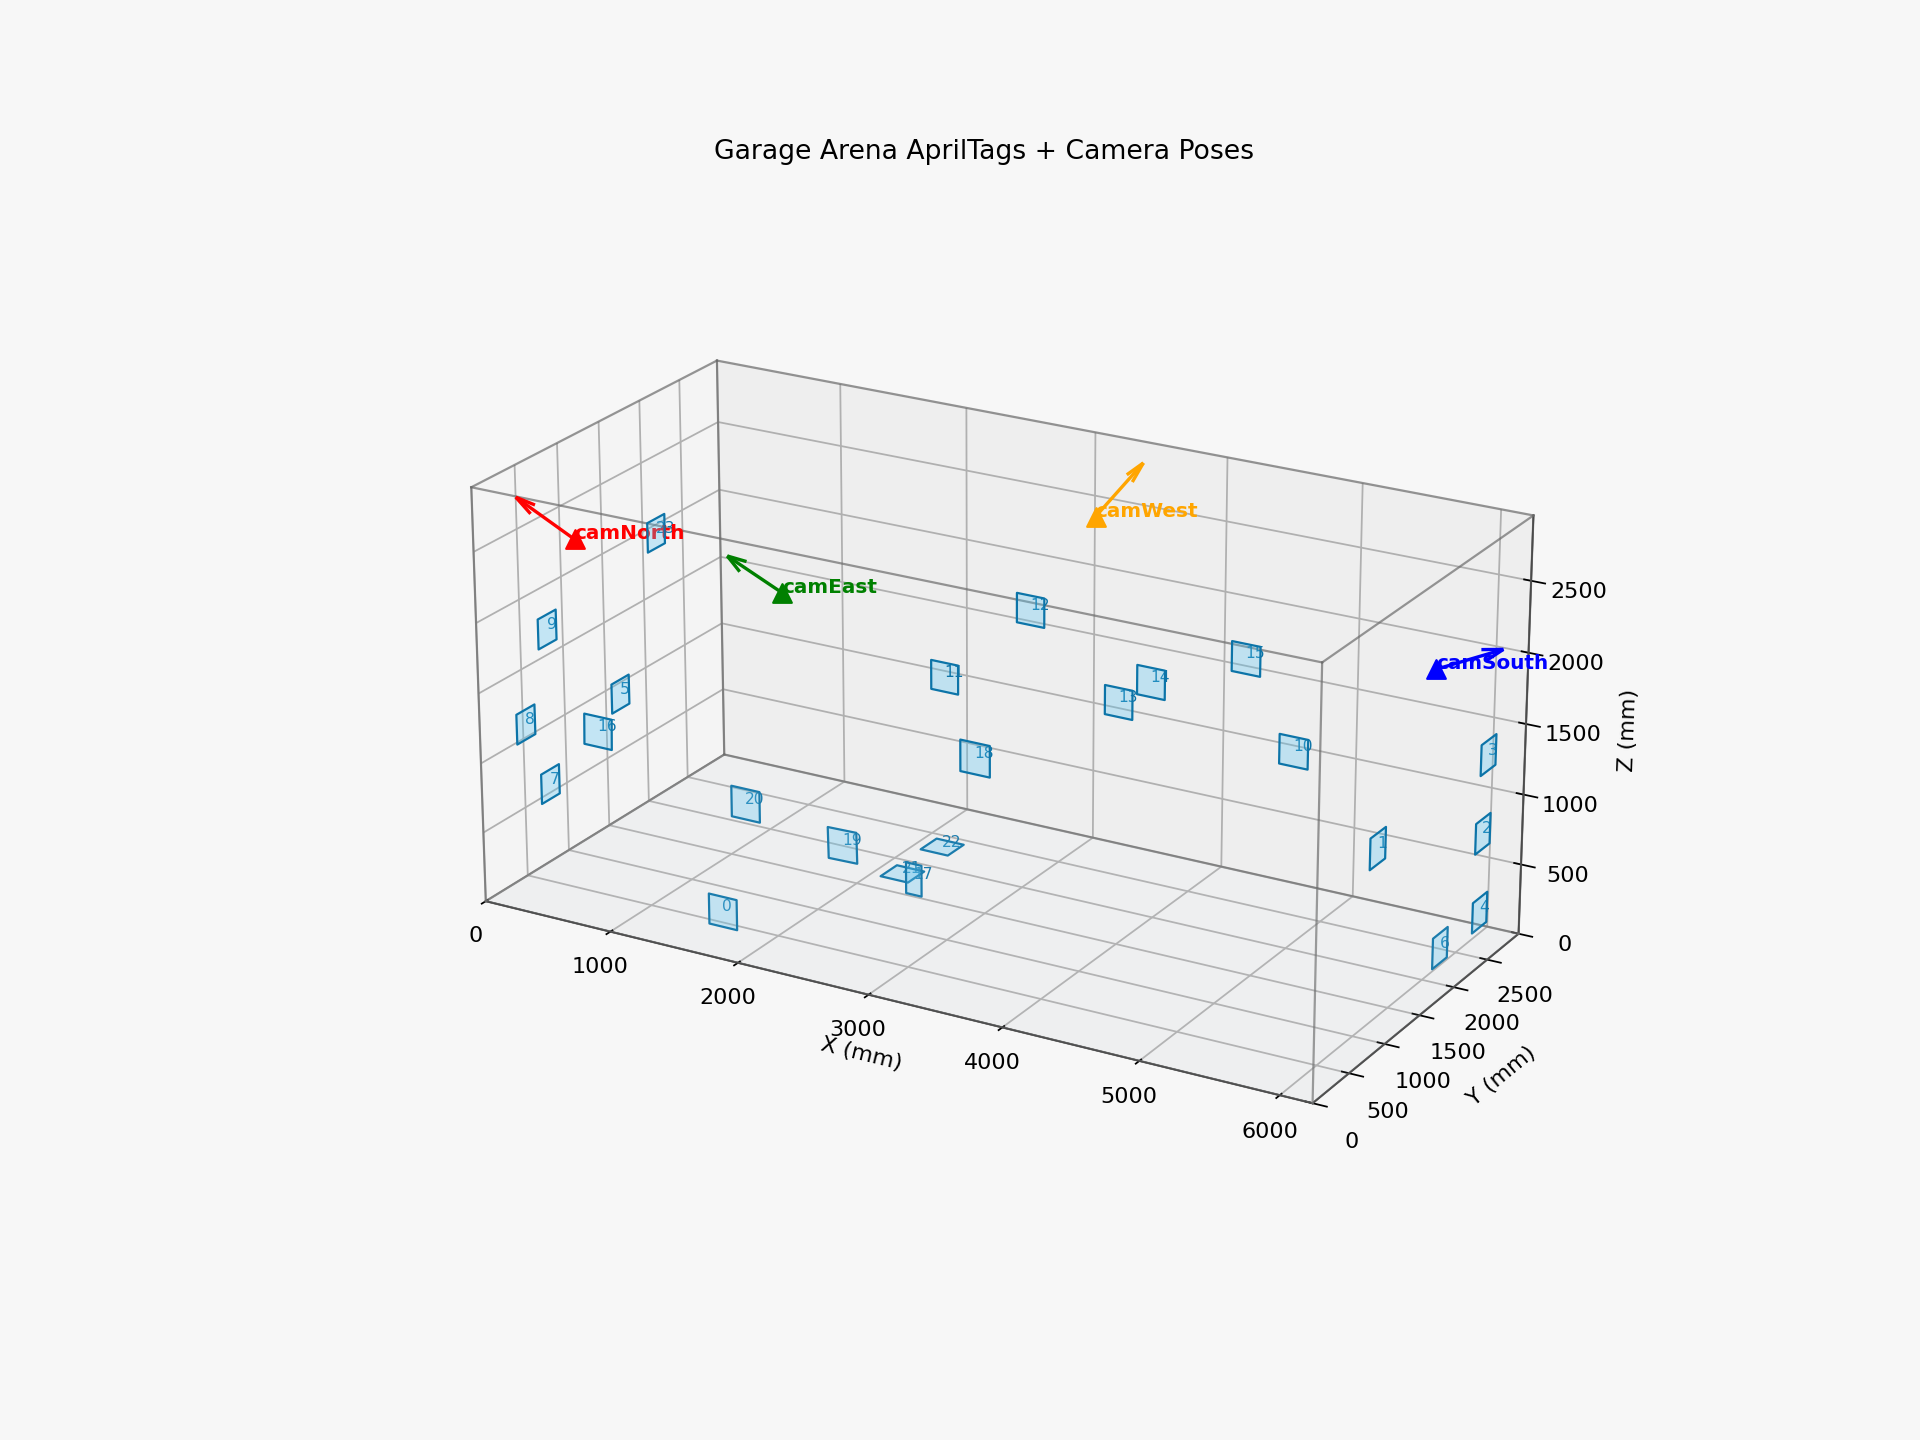
\includegraphics[width=0.9\textwidth]{figures/fig_arena360_view_01.png}
  \caption{Garage arena 3D reconstruction baseline view.}
  \label{fig:3_1_arena_baseline}
\end{figure}

\begin{figure}[htbp]
  \centering
  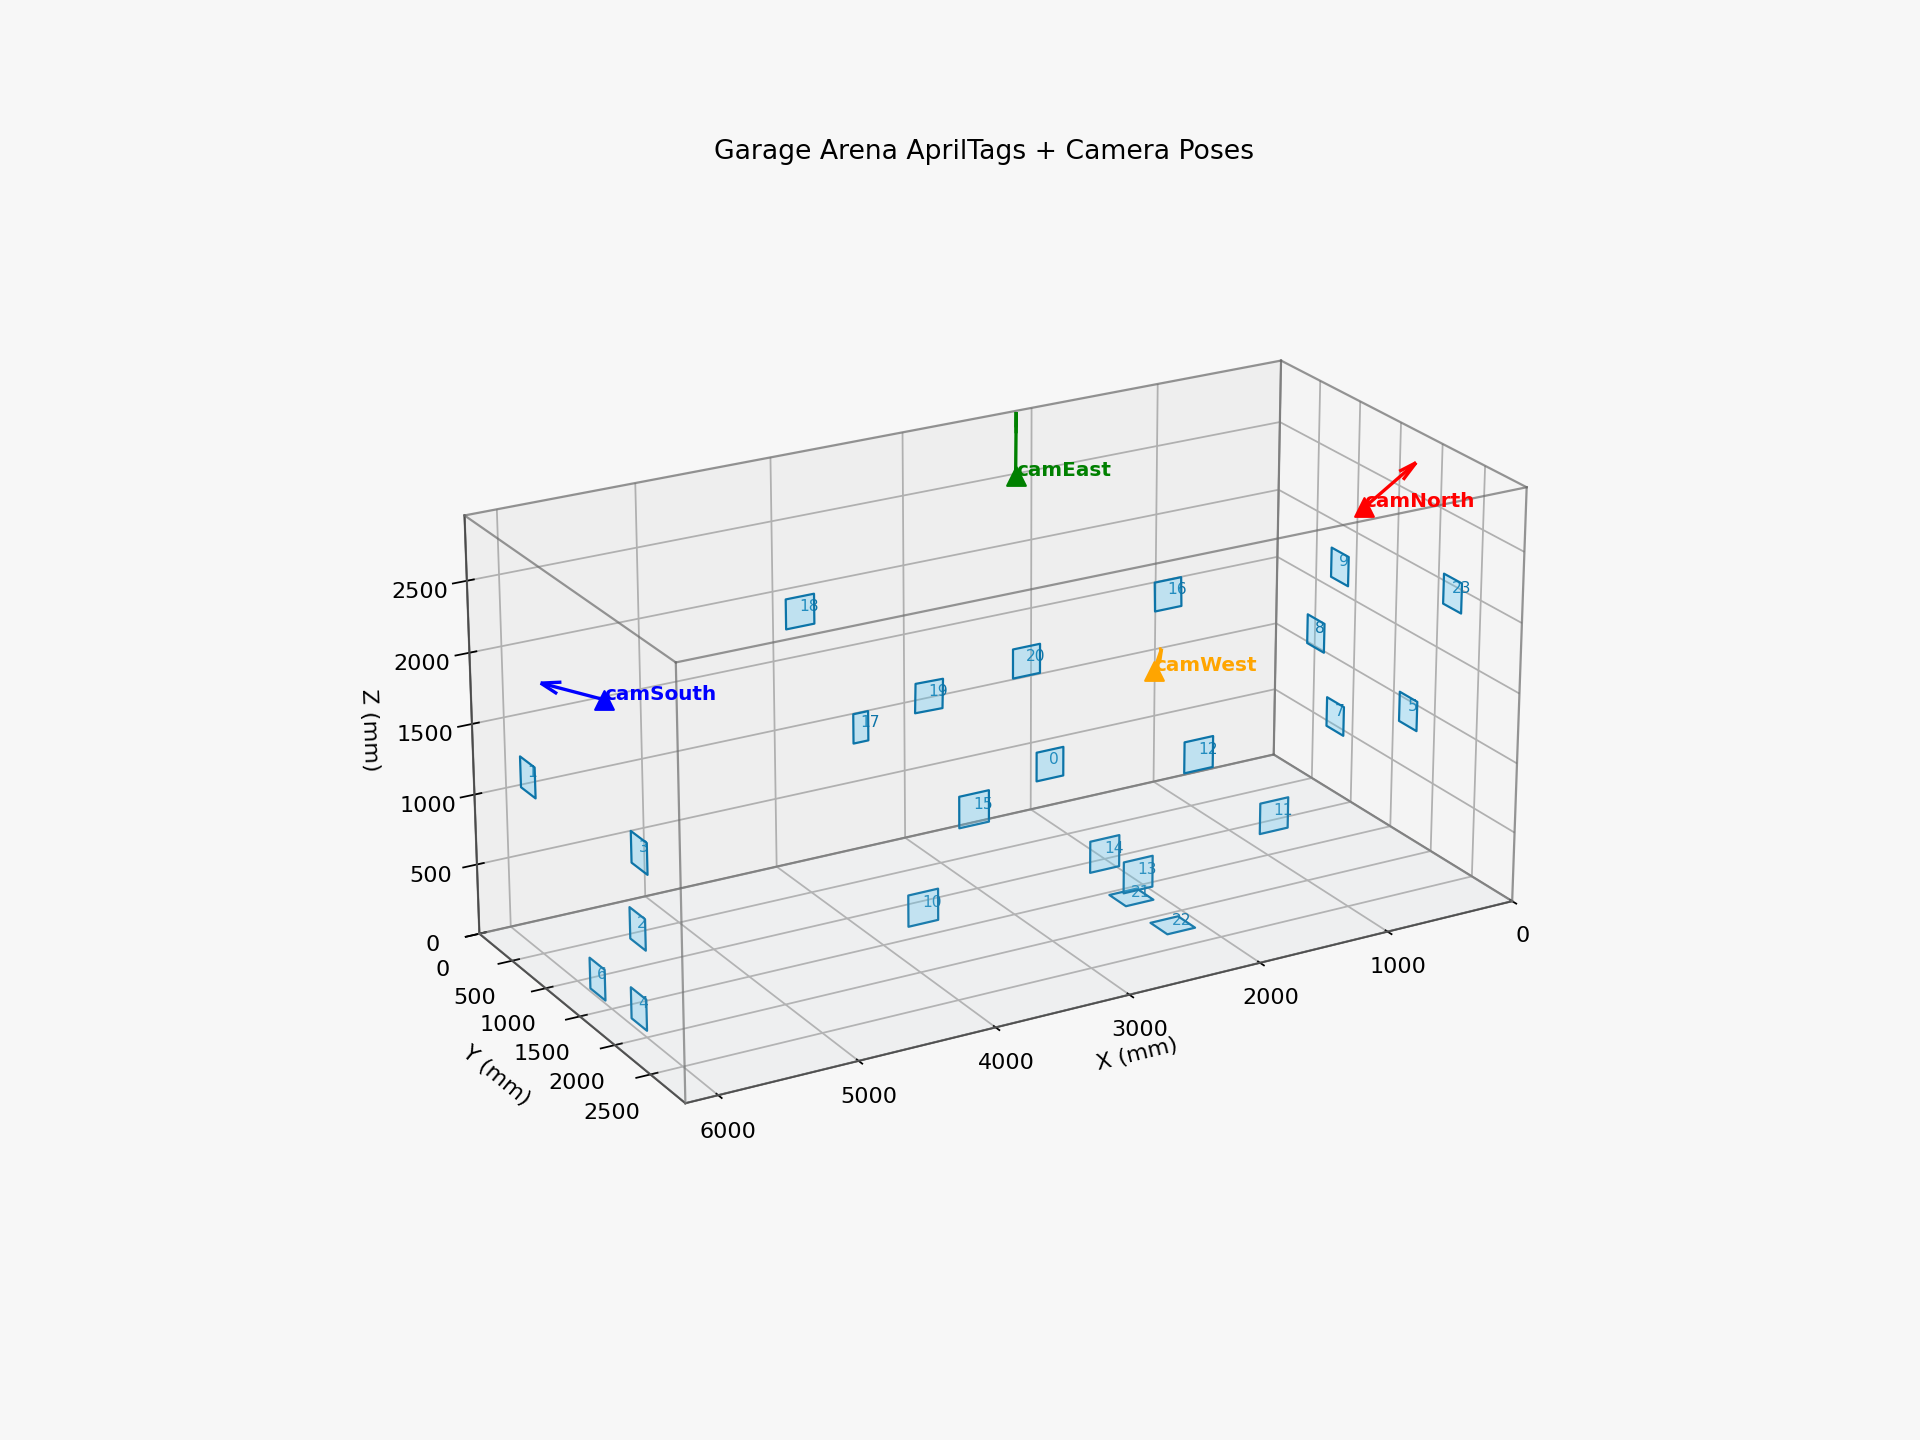
\includegraphics[width=0.9\textwidth]{figures/fig_arena360_view_02.png}
  \caption{Garage arena 3D reconstruction orbit view.}
  \label{fig:3_2_arena_orbit}
\end{figure}

\begin{figure}[htbp]
  \centering
  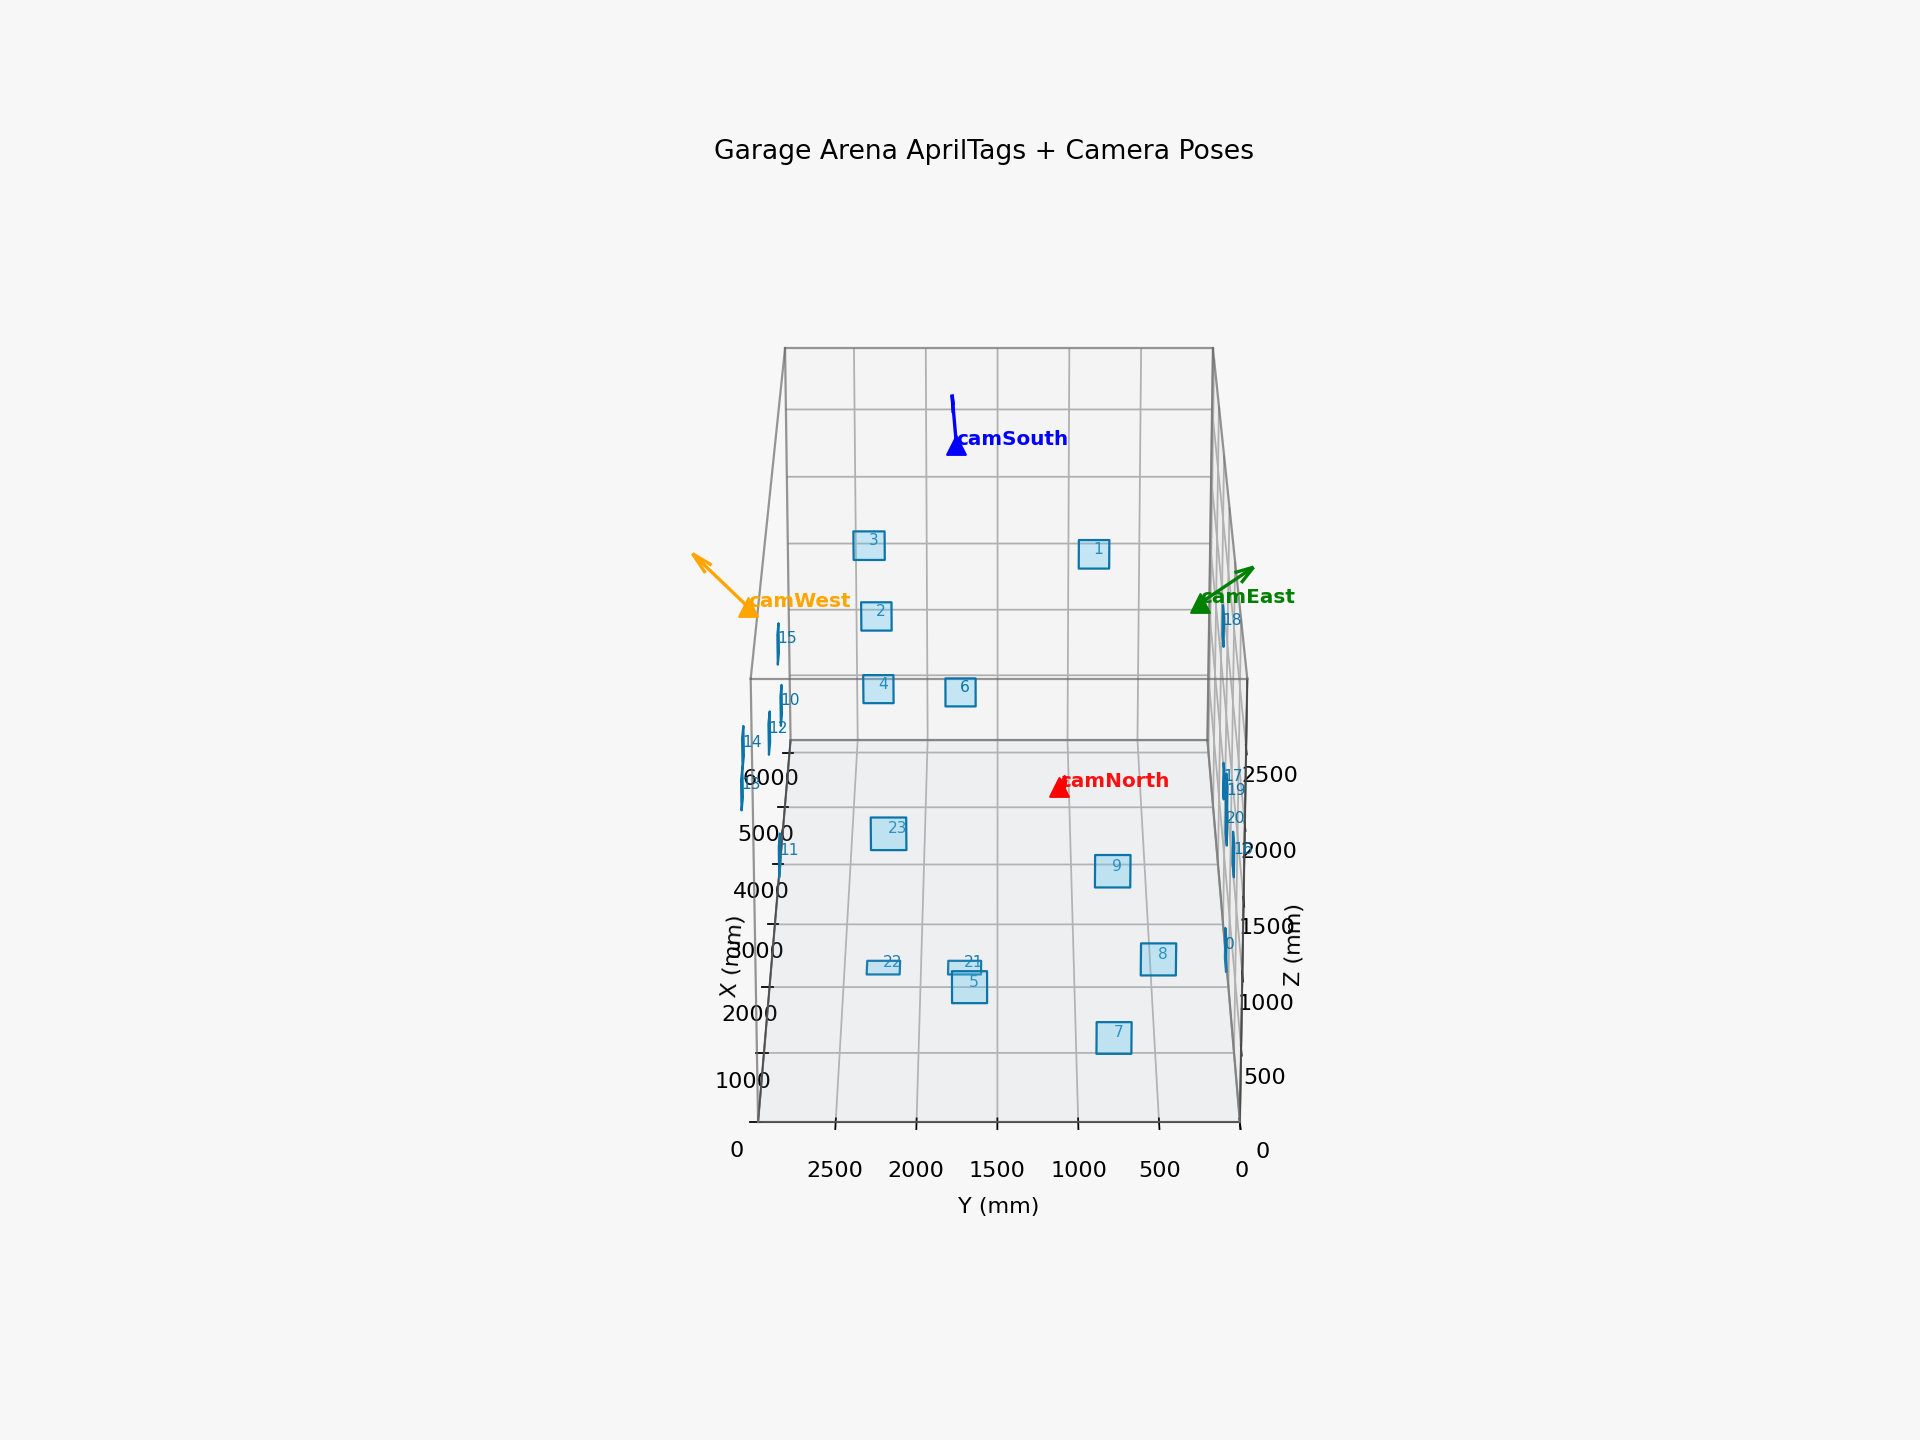
\includegraphics[width=0.9\textwidth]{figures/fig_arena360_view_03.png}
  \caption{Garage arena 3D reconstruction extended orbit view.}
  \label{fig:3_3_arena_orbit_extended}
\end{figure}

% Chapter 4 overlays
\begin{figure}[htbp]
  \centering
  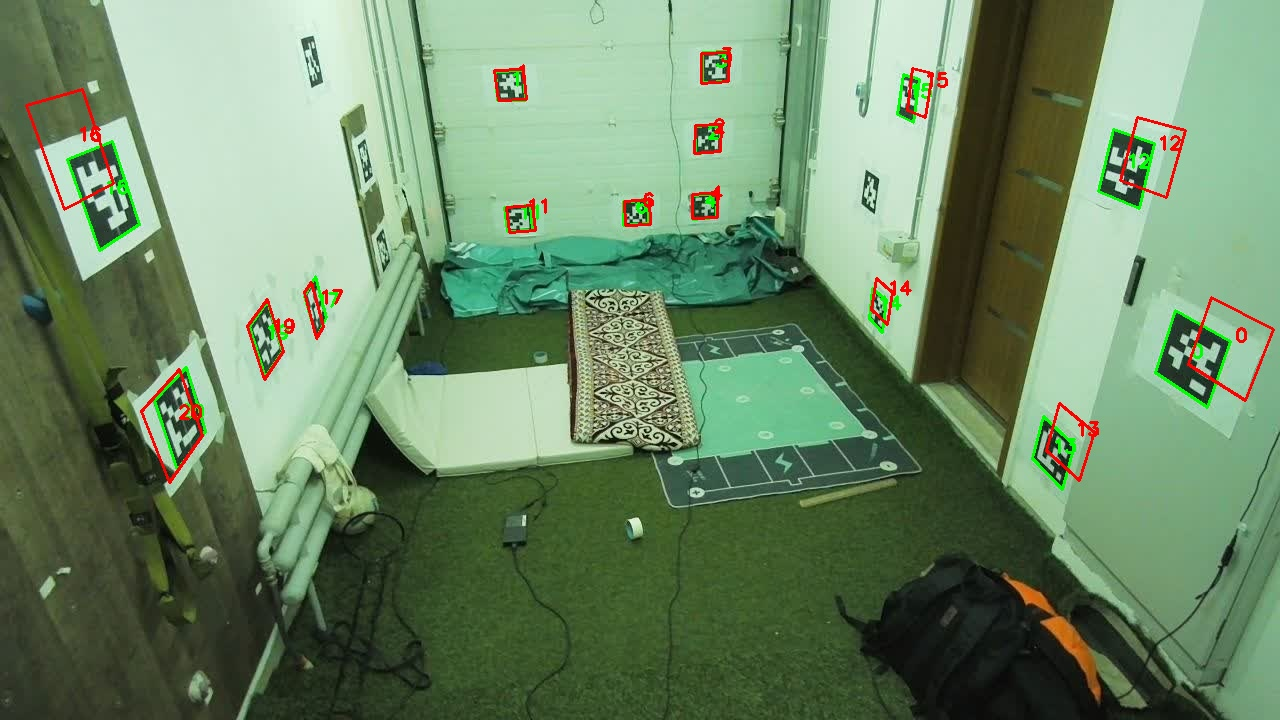
\includegraphics[width=0.8\textwidth]{figures/fig_overlay_camNorth.jpg}
  \caption{Extrinsics overlay validation for camNorth (detected vs projected corners).}
  \label{fig:4_1_overlay_north}
\end{figure}

\begin{figure}[htbp]
  \centering
  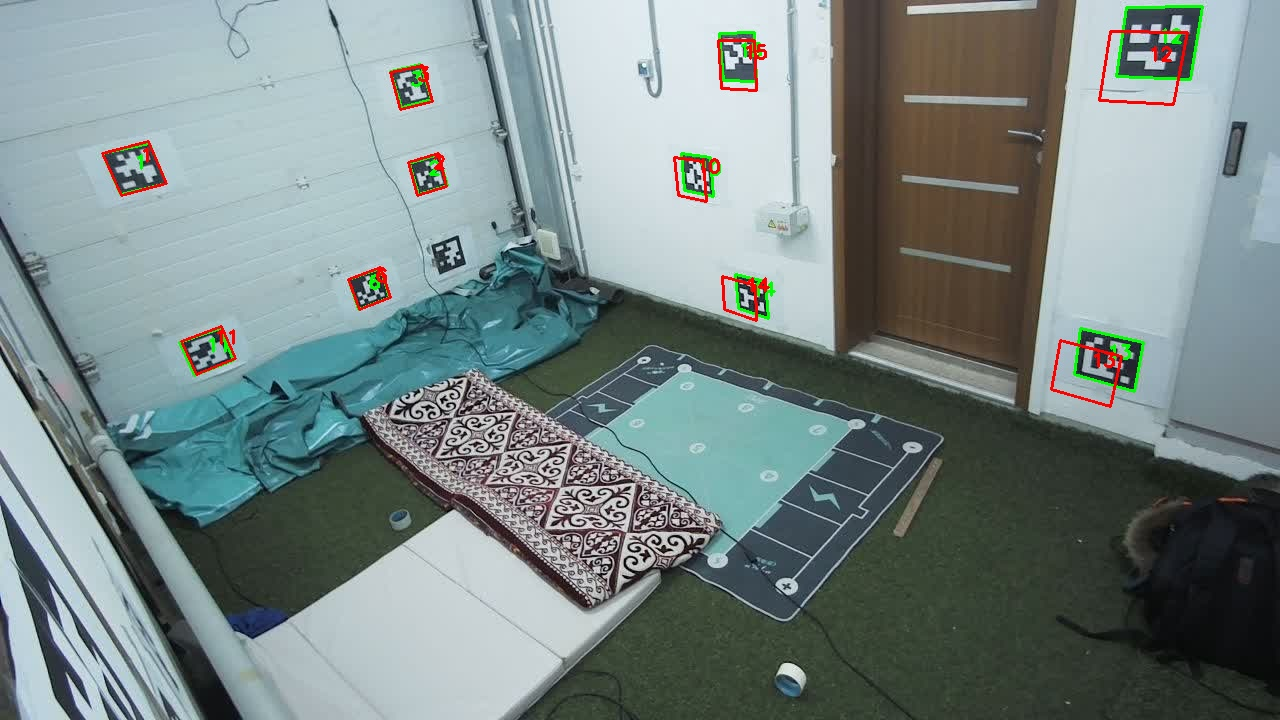
\includegraphics[width=0.8\textwidth]{figures/fig_overlay_camEast.jpg}
  \caption{Extrinsics overlay validation for camEast (detected vs projected corners).}
  \label{fig:4_2_overlay_east}
\end{figure}

\begin{figure}[htbp]
  \centering
  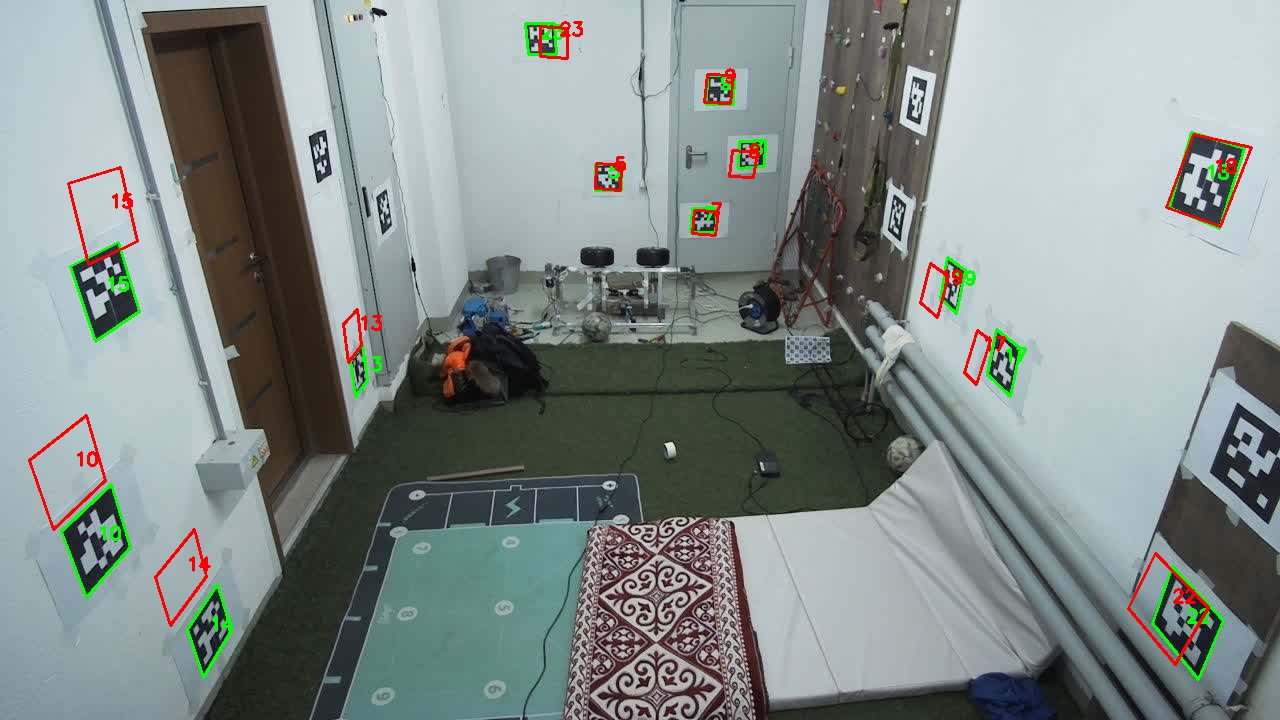
\includegraphics[width=0.8\textwidth]{figures/fig_overlay_camSouth.jpg}
  \caption{Extrinsics overlay validation for camSouth (detected vs projected corners).}
  \label{fig:4_3_overlay_south}
\end{figure}

\begin{figure}[htbp]
  \centering
  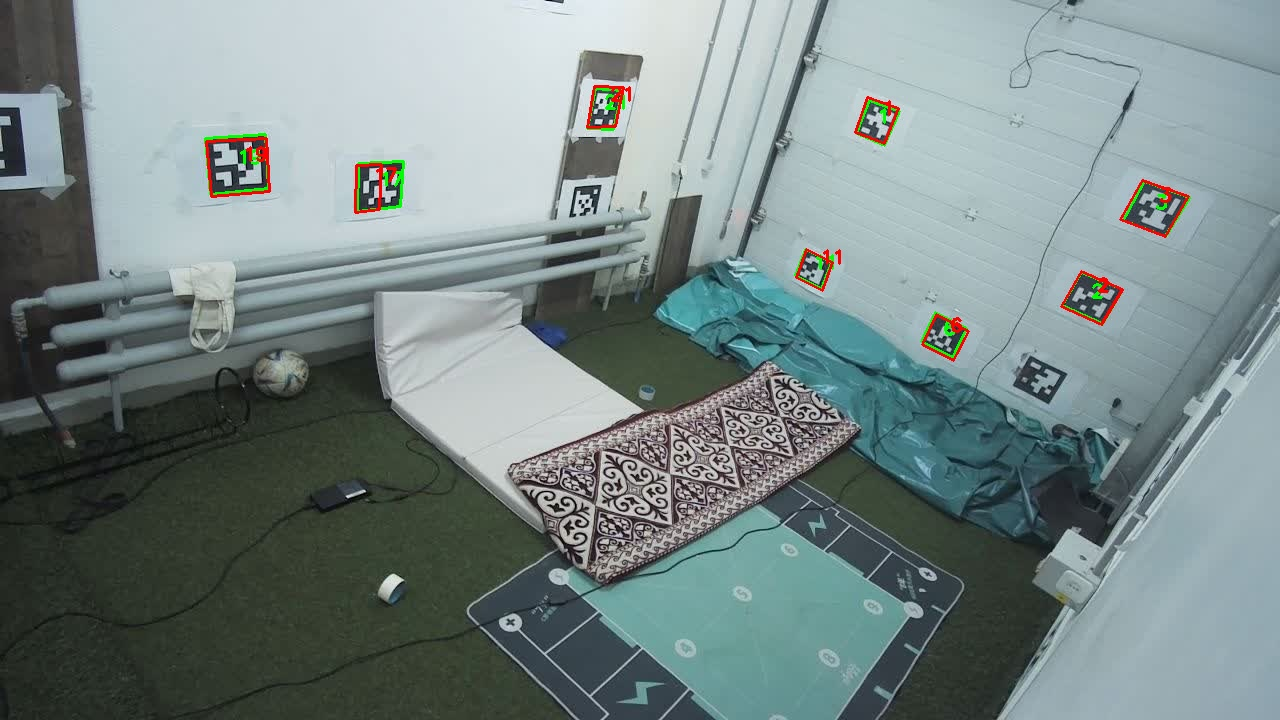
\includegraphics[width=0.8\textwidth]{figures/fig_overlay_camWest.jpg}
  \caption{Extrinsics overlay validation for camWest (detected vs projected corners).}
  \label{fig:4_4_overlay_west}
\end{figure}

% Chapter 5 smoke frames
\begin{figure}[htbp]
  \centering
  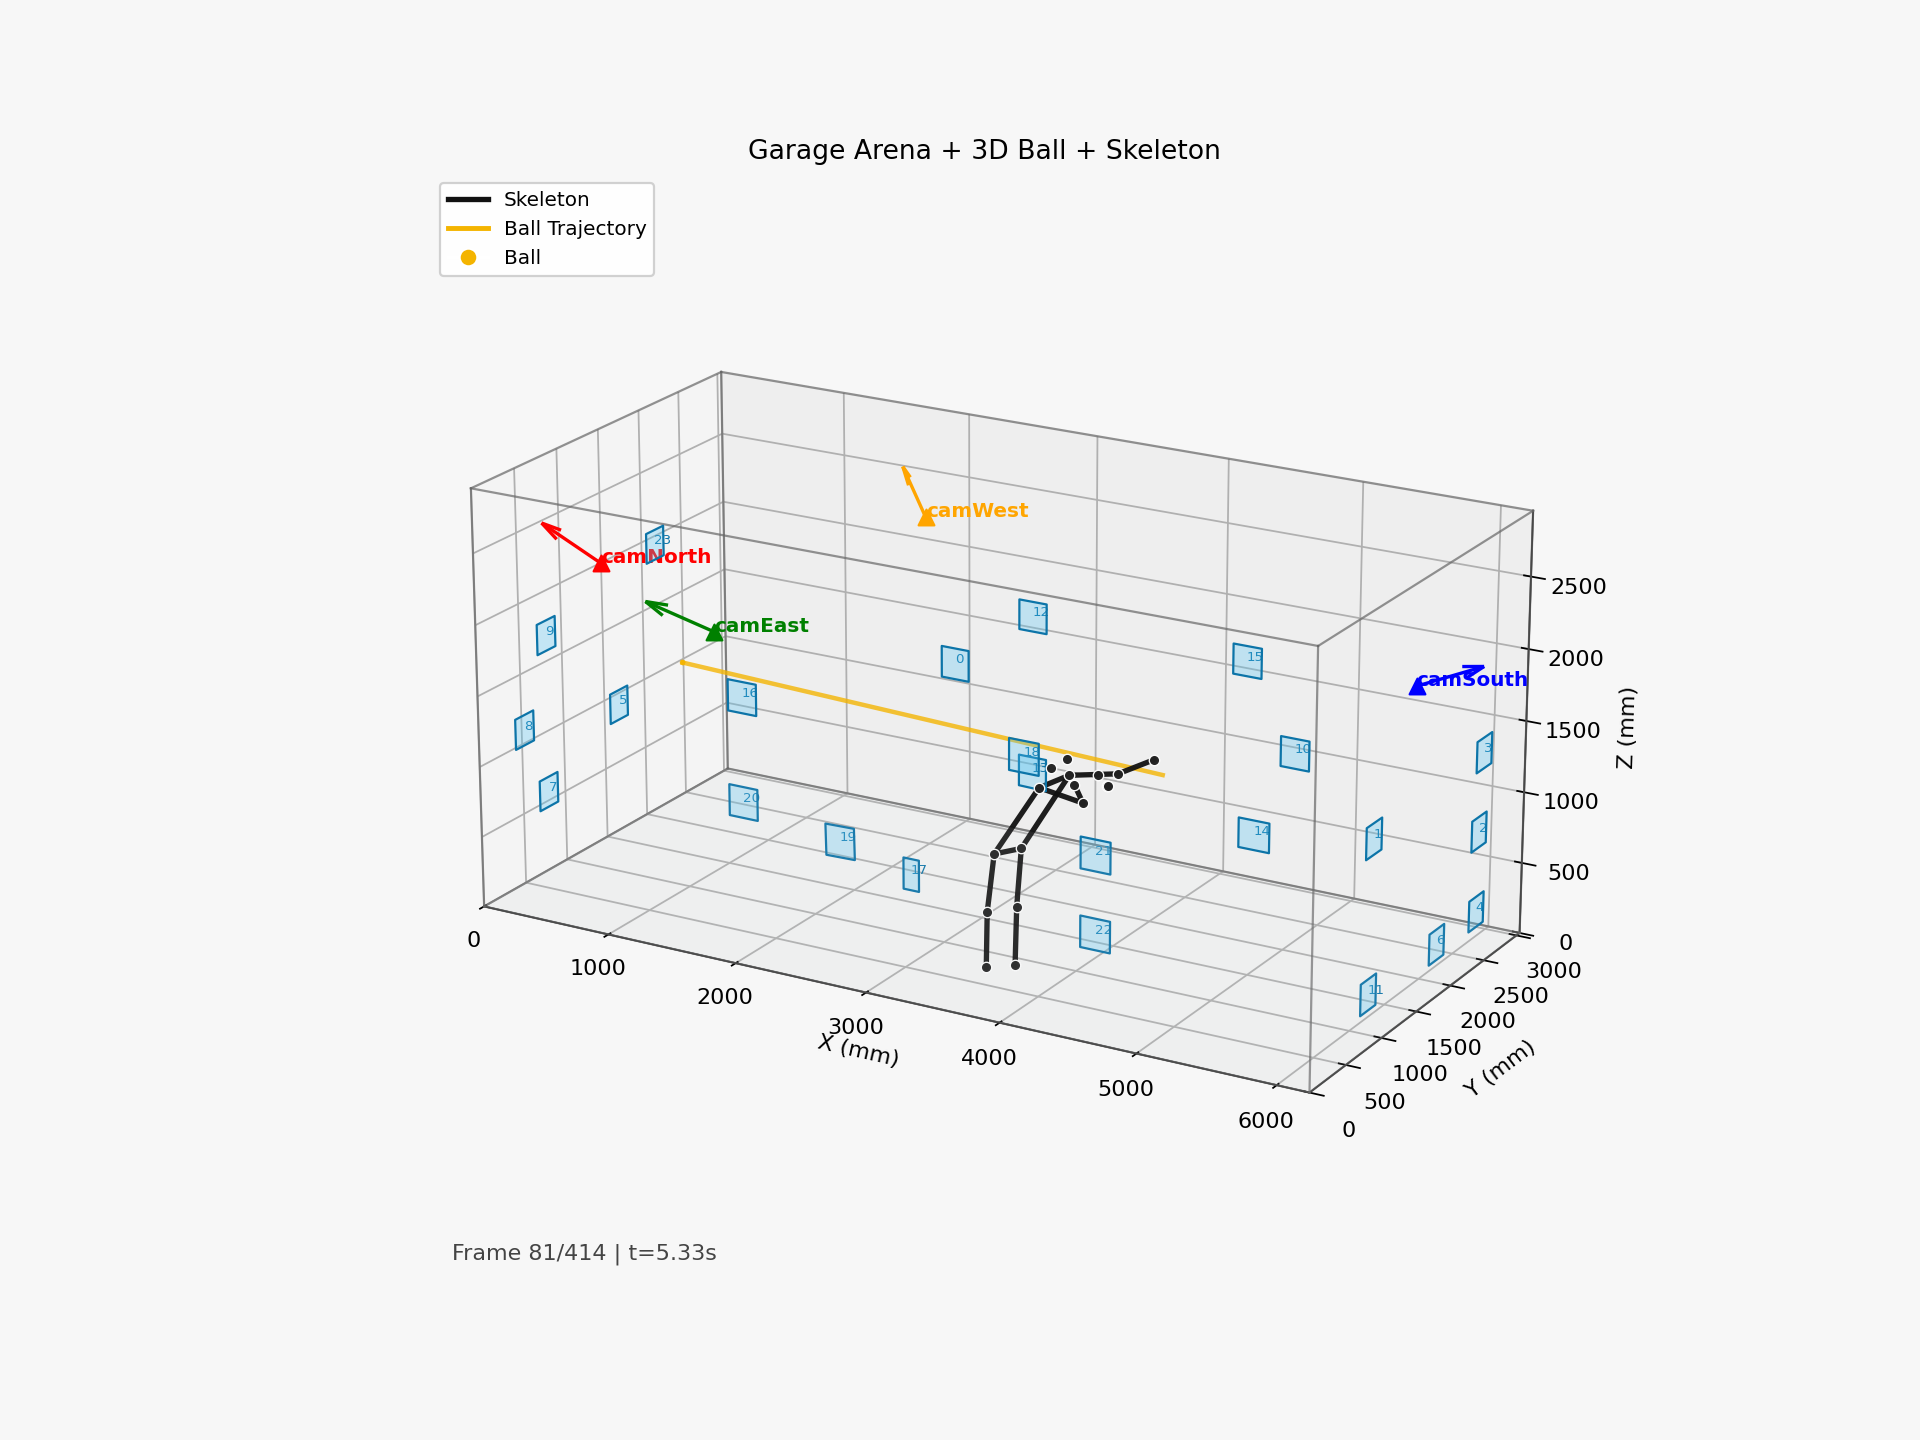
\includegraphics[width=0.9\textwidth]{figures/fig_smoke_frame_0080.png}
  \caption{Smoke session reconstructed frame 80.}
  \label{fig:5_1_smoke_80}
\end{figure}

\begin{figure}[htbp]
  \centering
  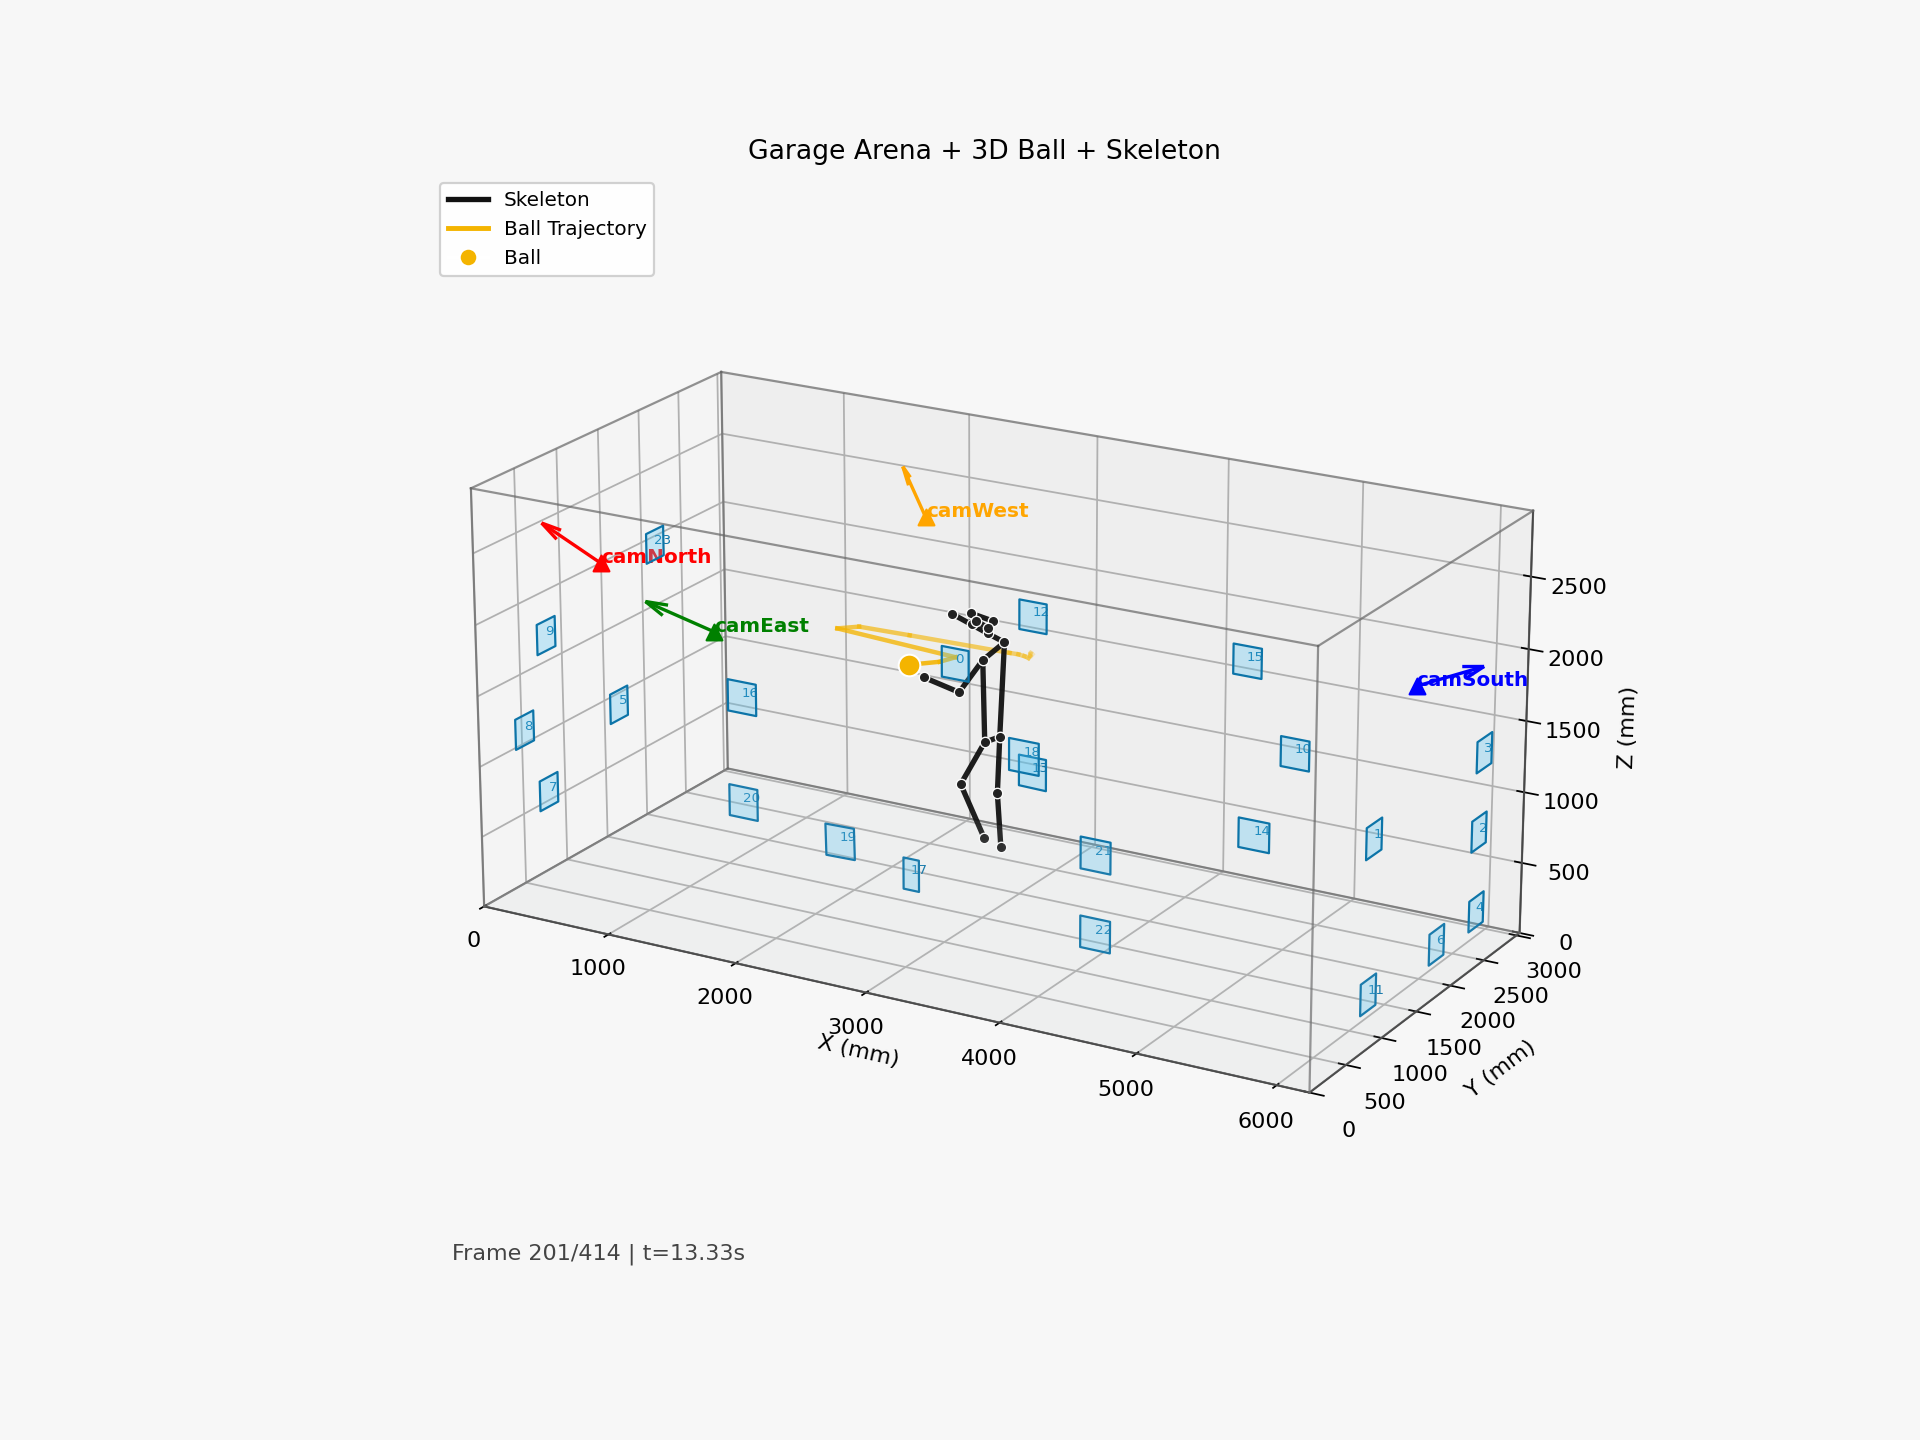
\includegraphics[width=0.9\textwidth]{figures/fig_smoke_frame_0200.png}
  \caption{Smoke session reconstructed frame 200.}
  \label{fig:5_2_smoke_200}
\end{figure}

\begin{figure}[htbp]
  \centering
  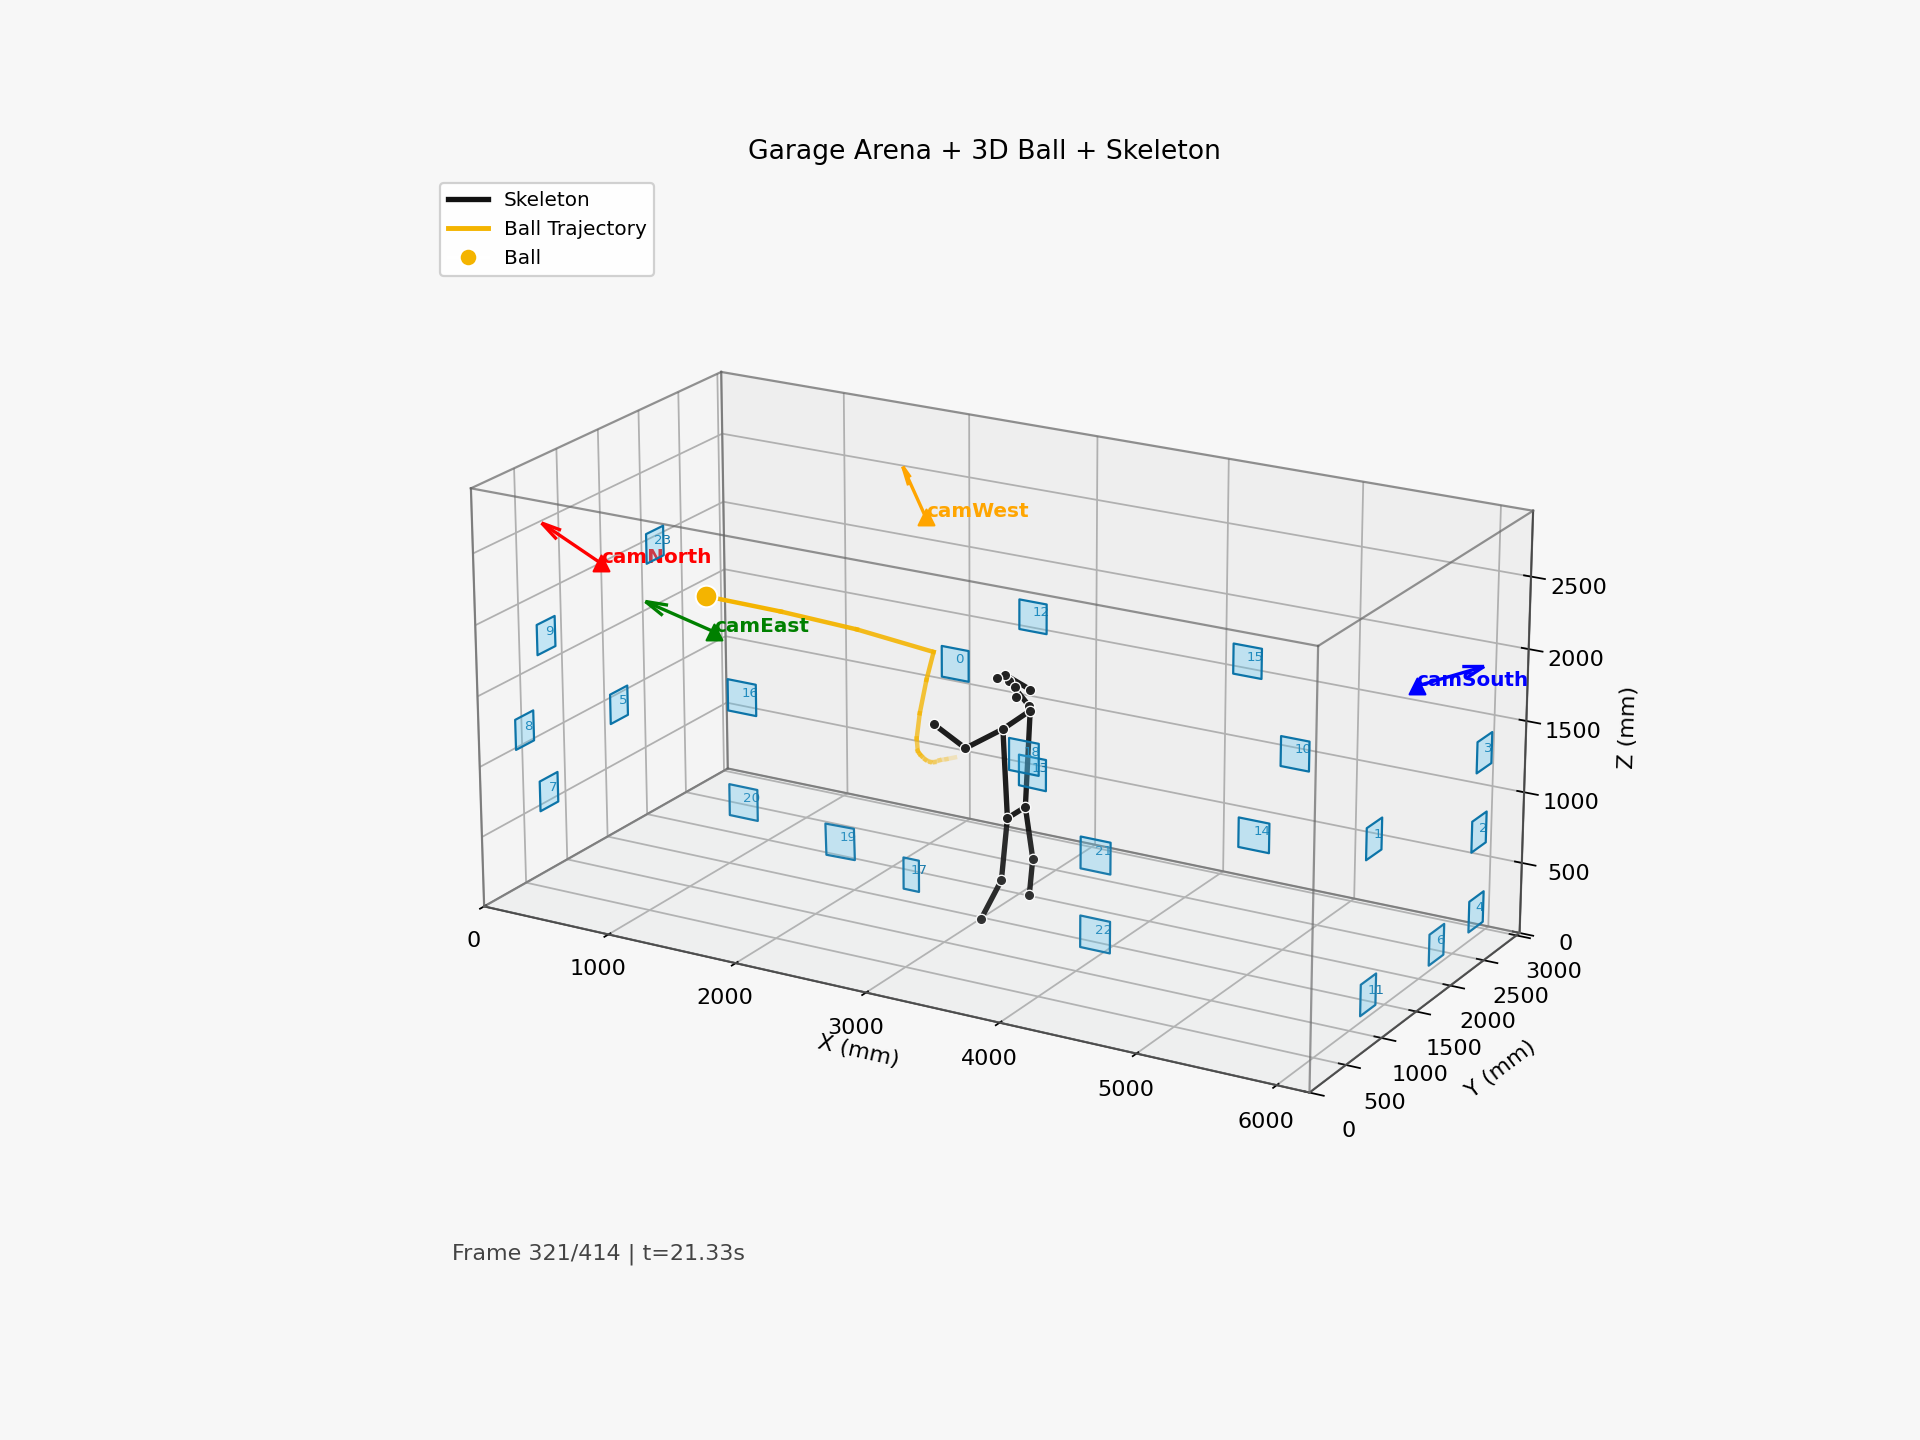
\includegraphics[width=0.9\textwidth]{figures/fig_smoke_frame_0320.png}
  \caption{Smoke session reconstructed frame 320.}
  \label{fig:5_3_smoke_320}
\end{figure}

% Chapter 7 metrics
\begin{figure}[htbp]
  \centering
  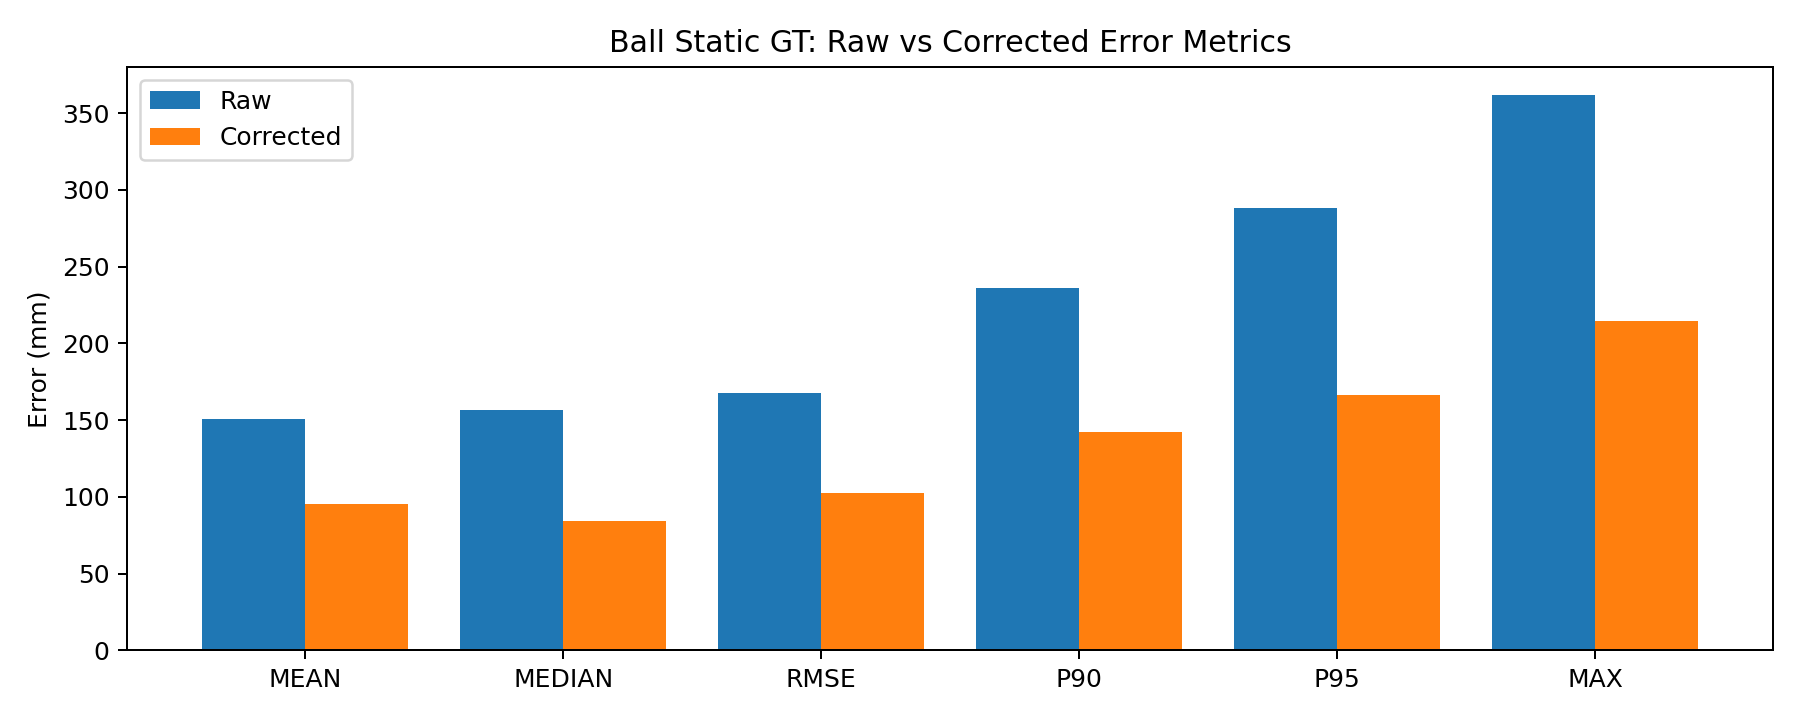
\includegraphics[width=0.95\textwidth]{figures/fig_static_raw_vs_corrected.png}
  \caption{Ball static GT error metrics before and after axis-wise correction.}
  \label{fig:7_1_static_raw_corrected}
\end{figure}

\begin{figure}[htbp]
  \centering
  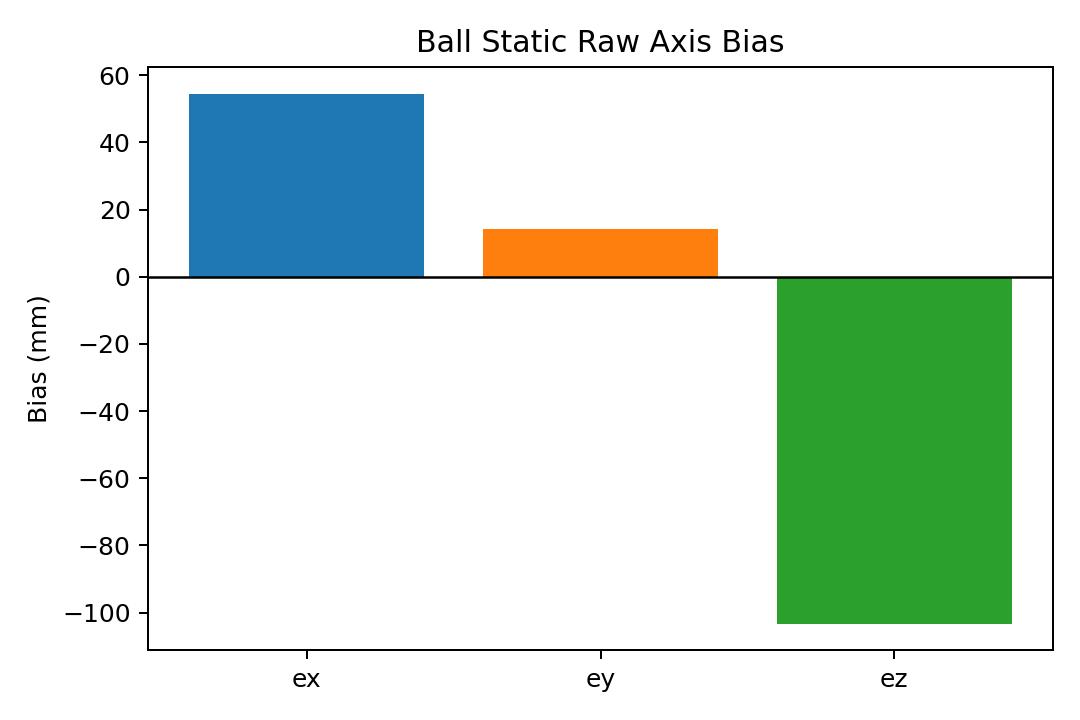
\includegraphics[width=0.8\textwidth]{figures/fig_static_axis_bias_raw.png}
  \caption{Axis-wise raw bias of static ball localization.}
  \label{fig:7_2_static_axis_bias}
\end{figure}

\begin{figure}[htbp]
  \centering
  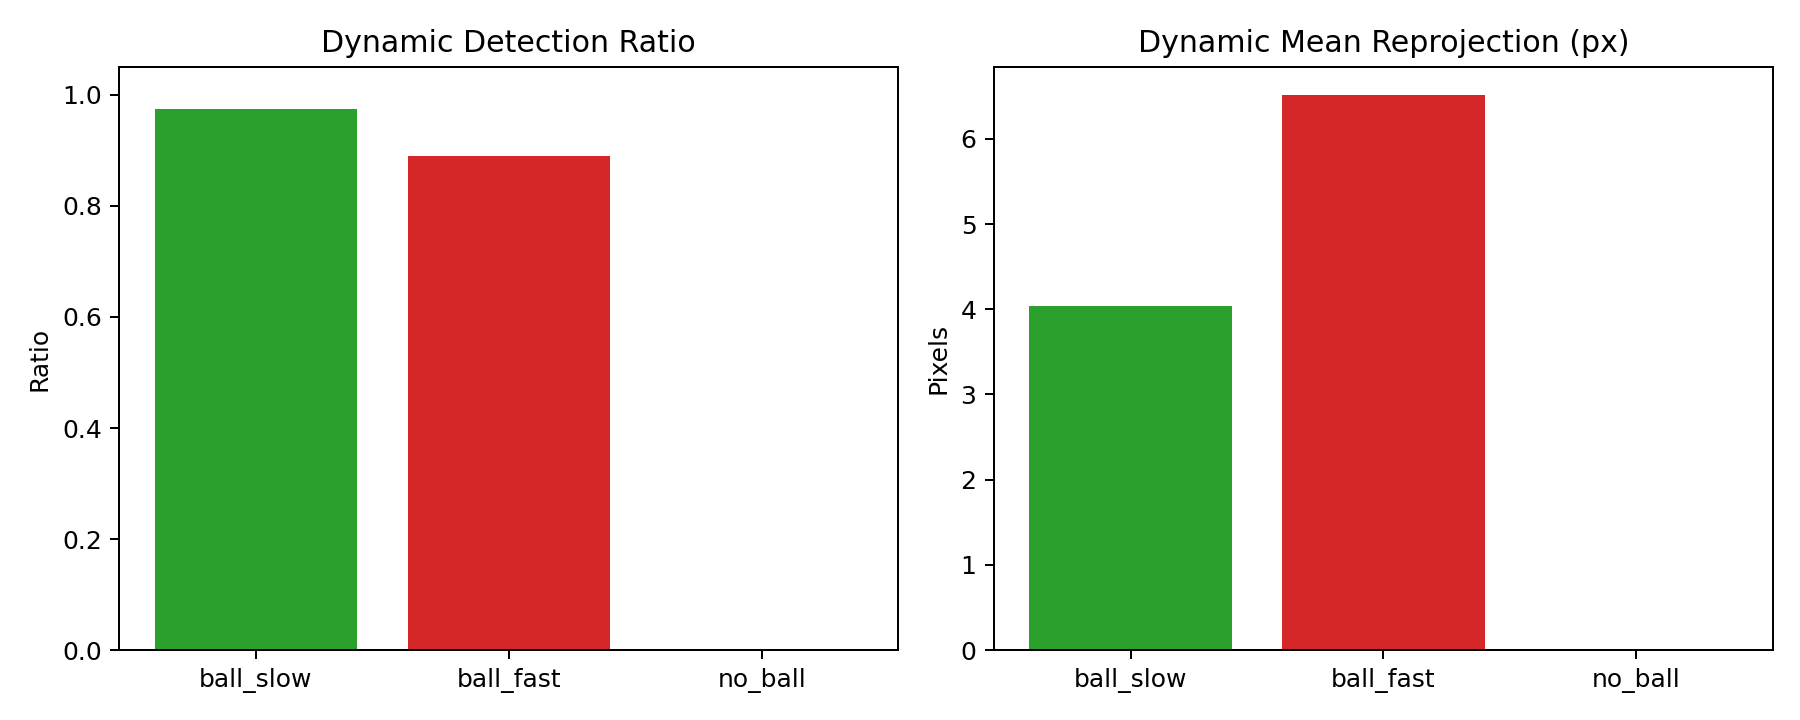
\includegraphics[width=0.95\textwidth]{figures/fig_dynamic_summary.png}
  \caption{Dynamic scenario summary: detection ratio and reprojection error.}
  \label{fig:7_3_dynamic_summary}
\end{figure}

\begin{figure}[htbp]
  \centering
  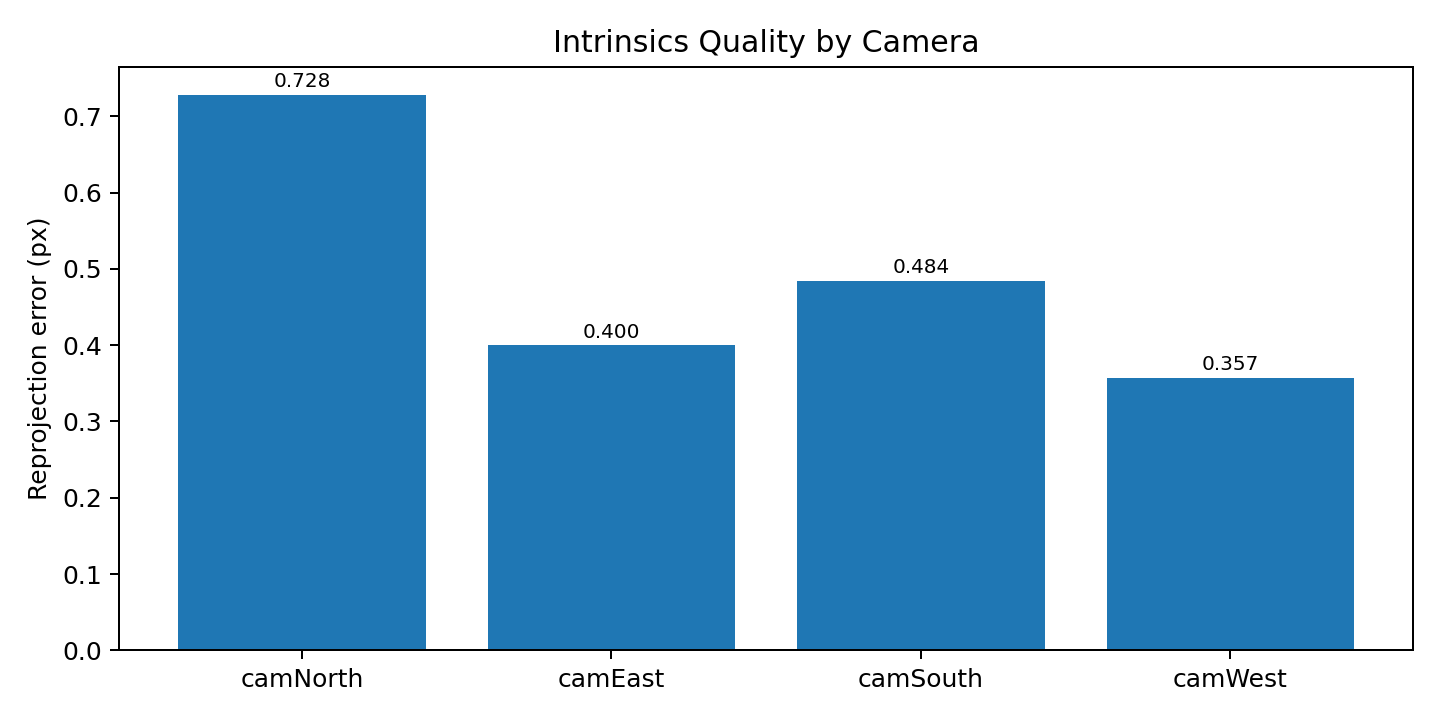
\includegraphics[width=0.85\textwidth]{figures/fig_intrinsics_reproj_by_camera.png}
  \caption{Intrinsics reprojection error by camera.}
  \label{fig:7_4_intrinsics_by_camera}
\end{figure}

\begin{figure}[htbp]
  \centering
  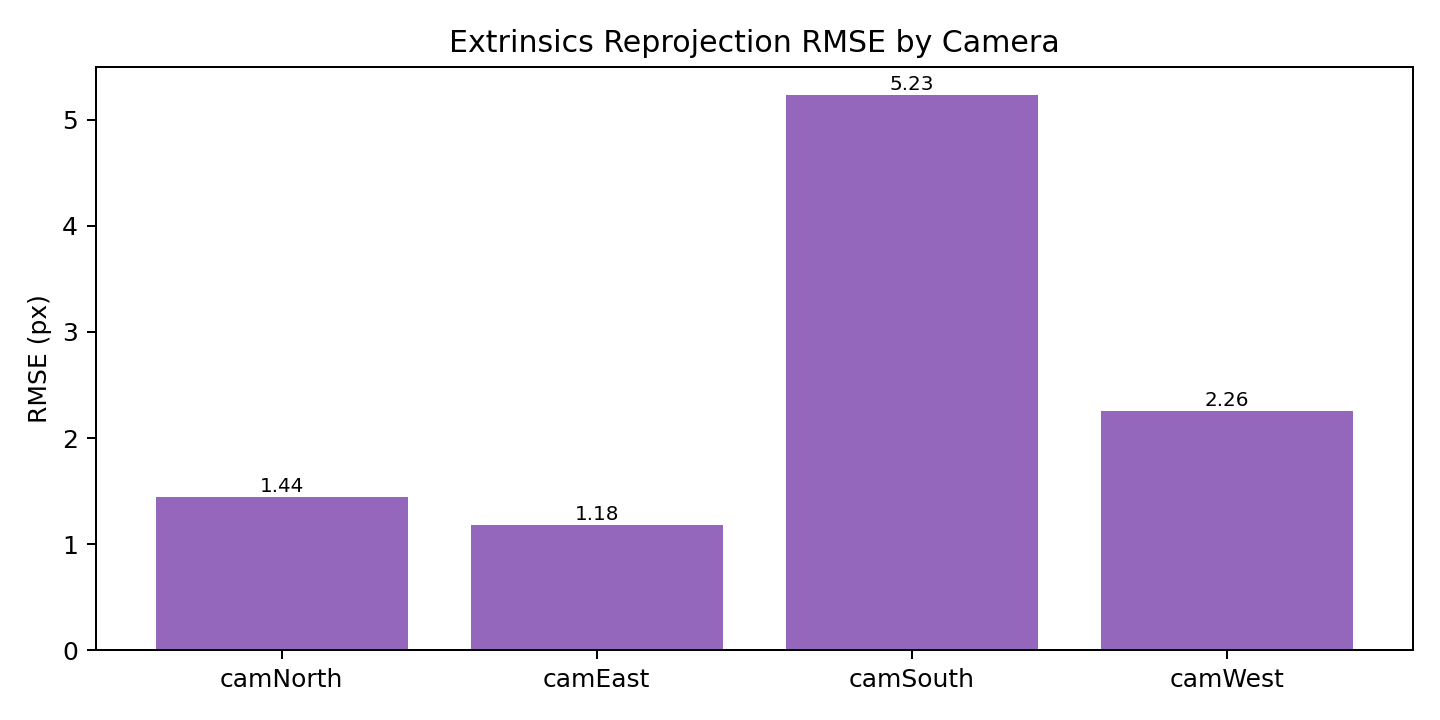
\includegraphics[width=0.85\textwidth]{figures/fig_extrinsics_rmse_by_camera.png}
  \caption{Extrinsics reprojection RMSE by camera.}
  \label{fig:7_5_extrinsics_by_camera}
\end{figure}

\begin{figure}[htbp]
  \centering
  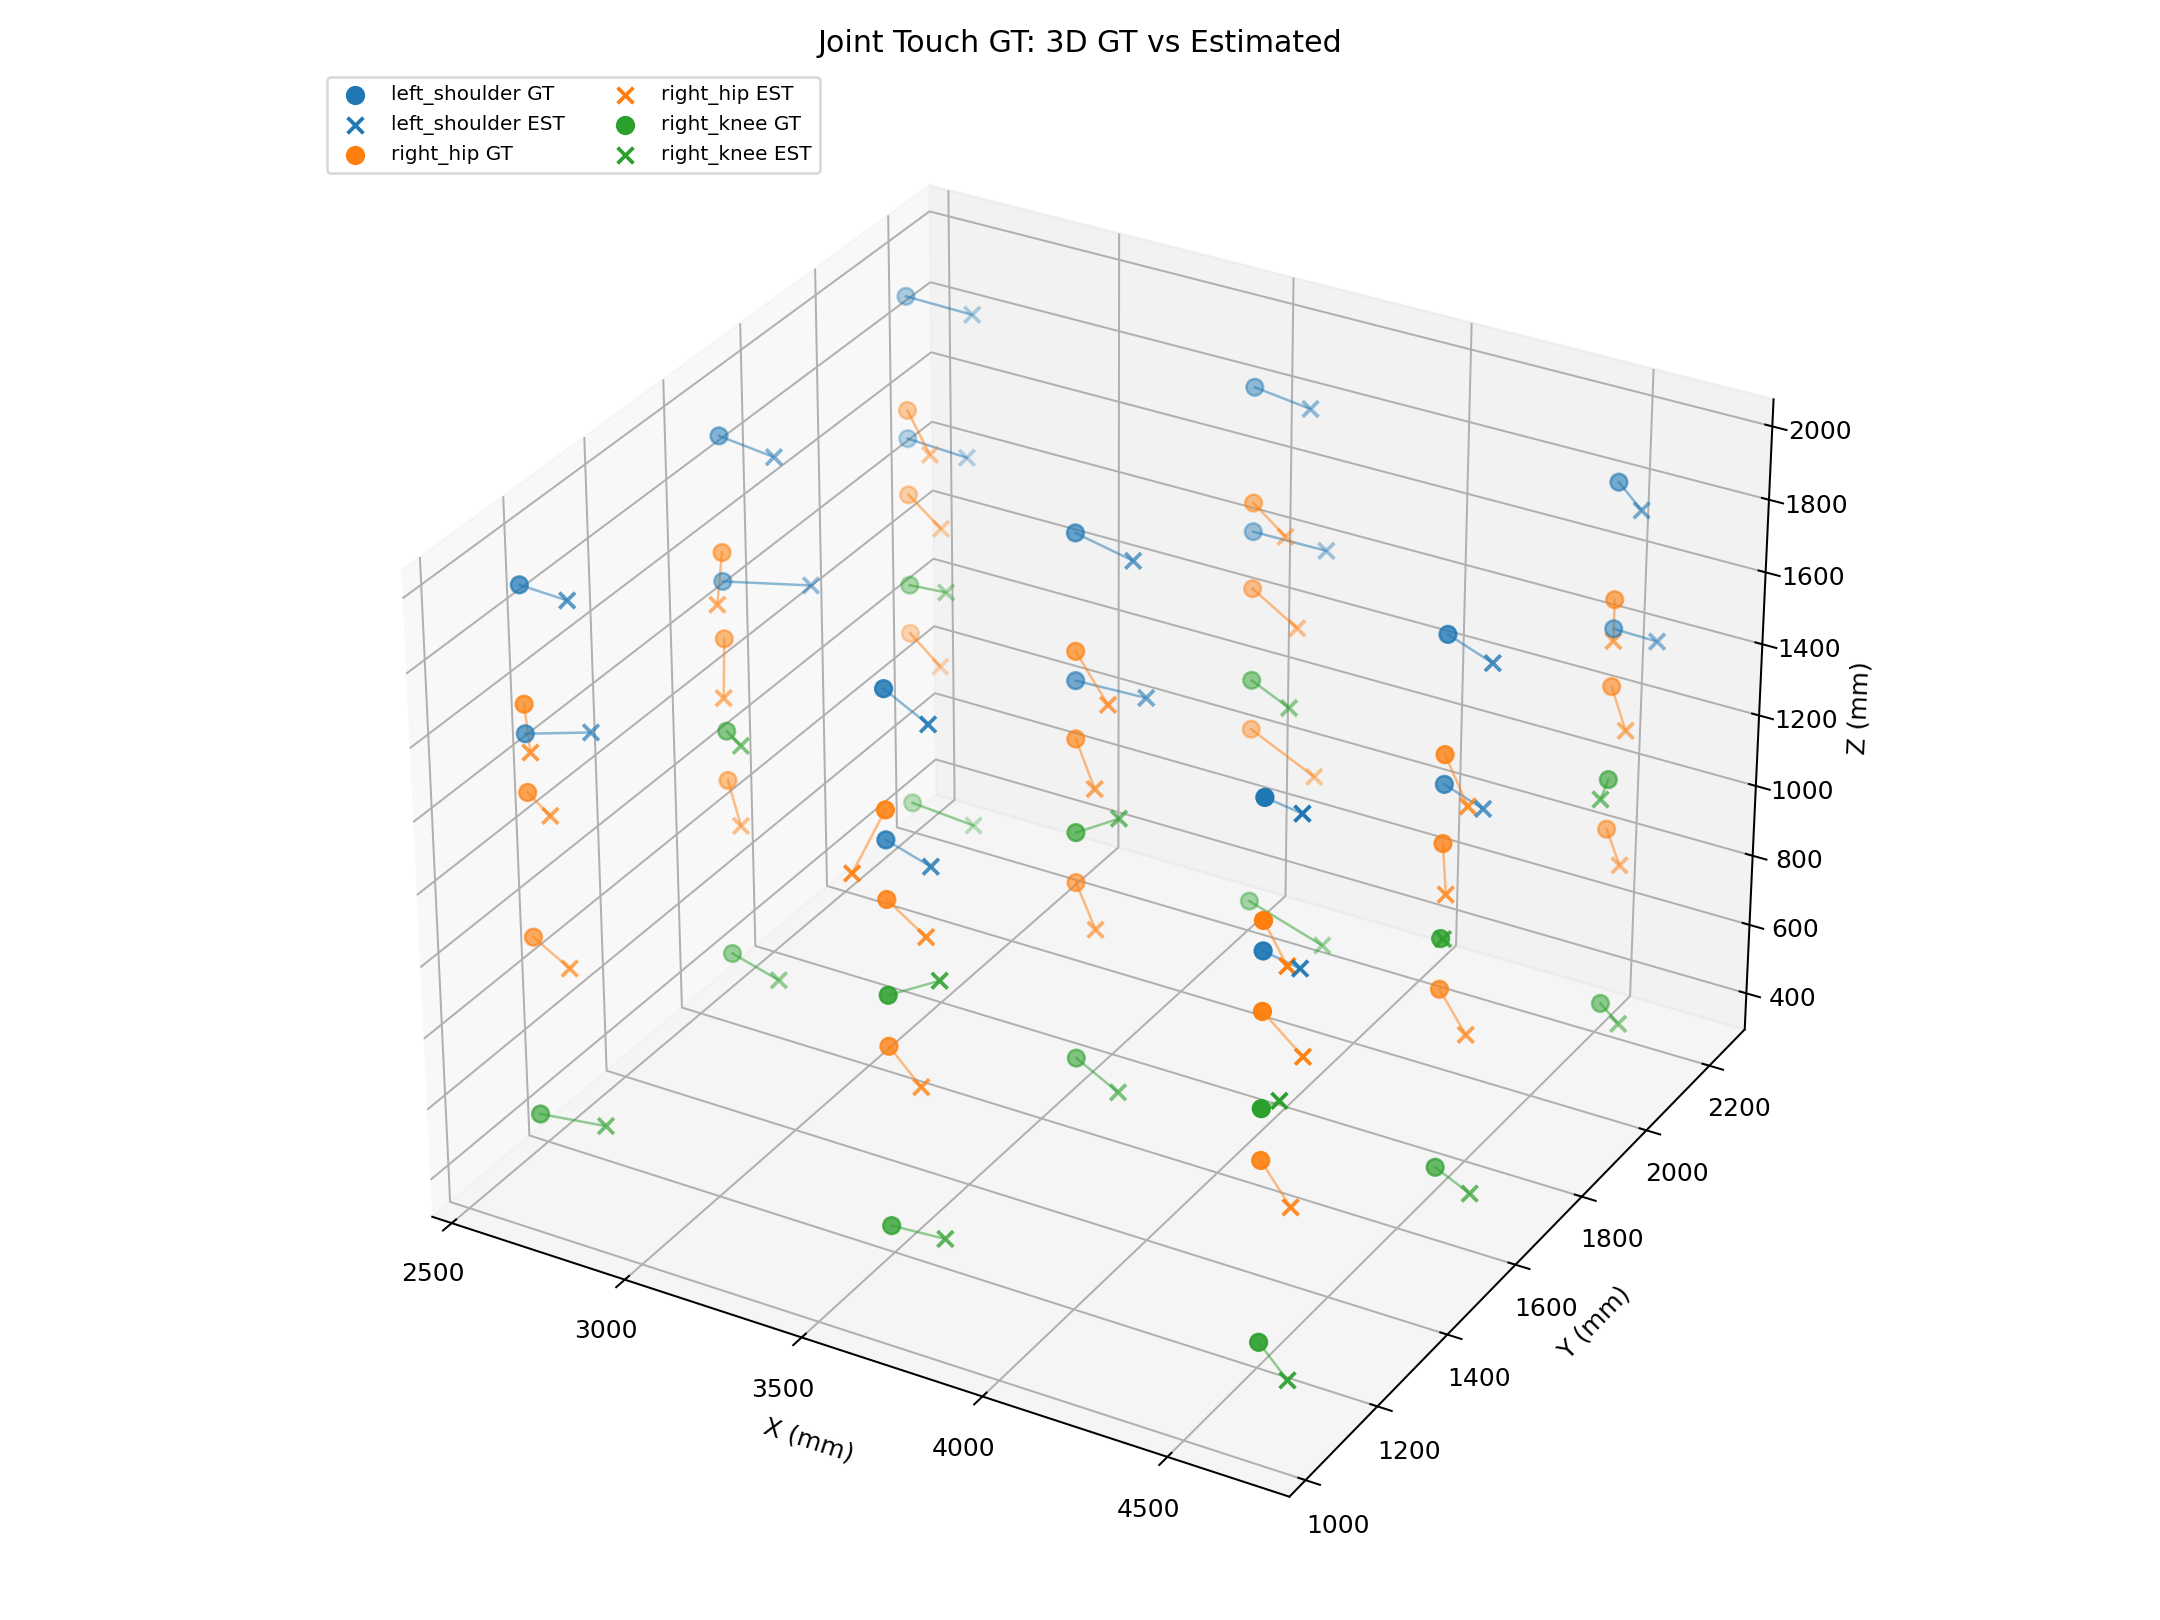
\includegraphics[width=0.95\textwidth]{figures/fig_joint_touch_3d_gt_vs_est.png}
  \caption{Joint-touch GT versus estimated 3D points.}
  \label{fig:7_6_joint_3d_gt_vs_est}
\end{figure}

\begin{figure}[htbp]
  \centering
  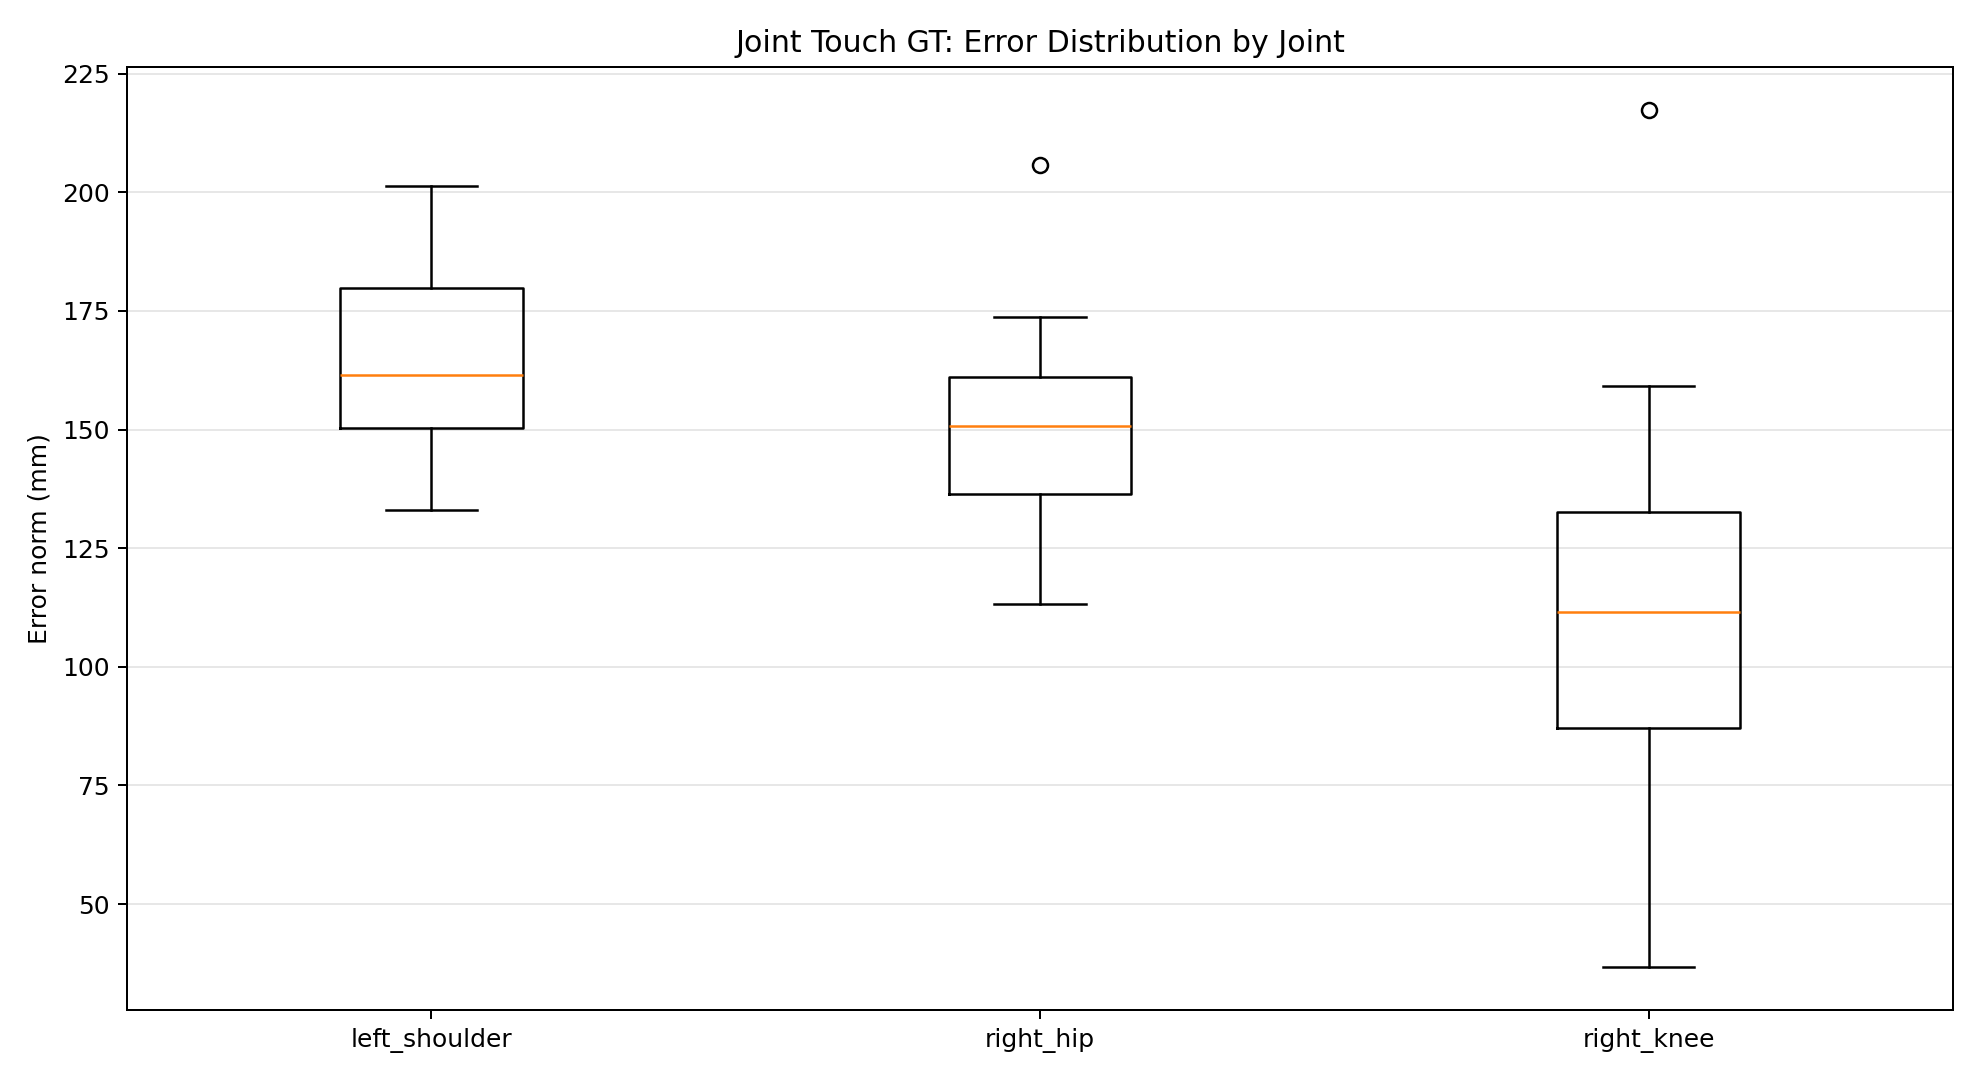
\includegraphics[width=0.8\textwidth]{figures/fig_joint_touch_error_boxplot.png}
  \caption{Joint-touch error distribution boxplot.}
  \label{fig:7_7_joint_error_boxplot}
\end{figure}

\begin{figure}[htbp]
  \centering
  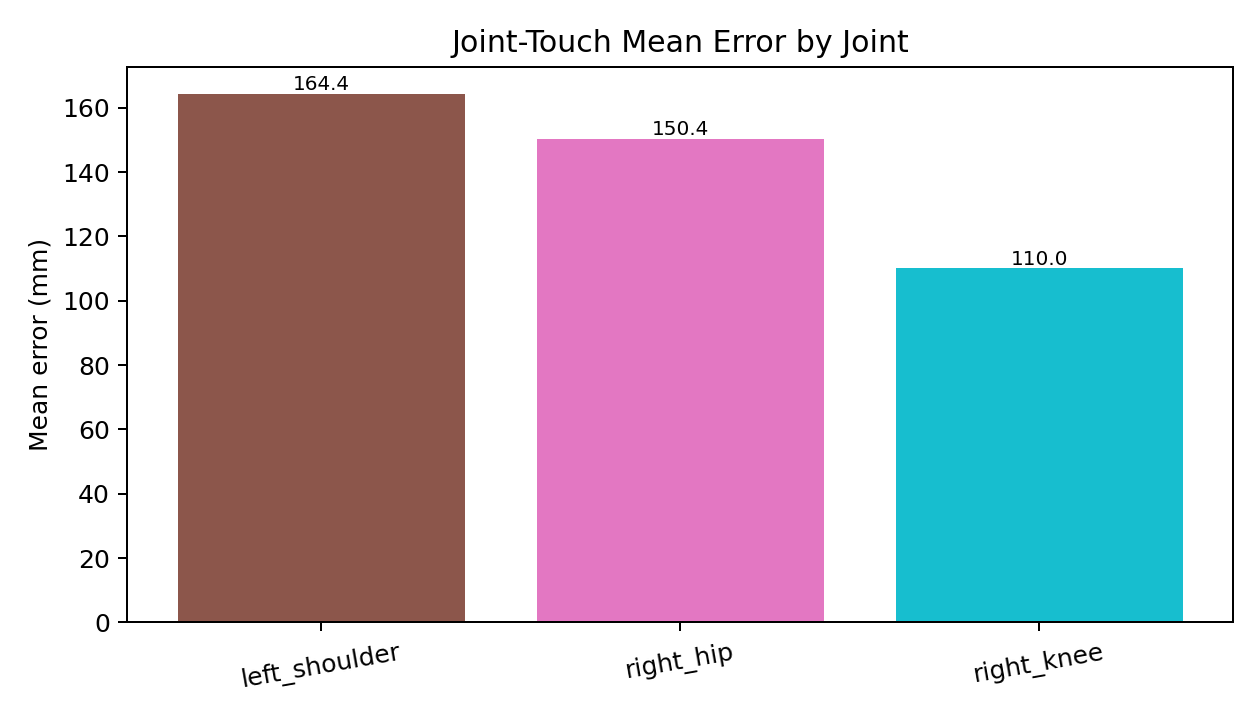
\includegraphics[width=0.8\textwidth]{figures/fig_joint_mean_error_by_joint.png}
  \caption{Mean joint localization error by joint class.}
  \label{fig:7_8_joint_mean}
\end{figure}
